\chapter{Temperature distribution of an idealized geological intrusion}

\modinfo{Directory}{HeatIntrusion1D}
\modinfo{Solvers}{\Idx{HeatSolve}} 
\modinfo{Tools}{\Idx{ElmerGUI}} 
\modinfo{Dimensions}{2D, Transient}
\modinfo{Author}{Peter R{\aa}back, Thomas Zwinger}


\subsection*{Problem description}

This is an extreme simplification of the intrusion process in 
related to geological processes. The case is effectively 1D but 
it is treated as 2D for generality of the approach. 

We study temperature distribution from -8~km to -4~km. It is assumed
that before the intrusion there is a linear temperature distribution
from 320 to 160 C. At $t=0$ an intrusion of 900 C replaces the 
temperature from -6.5~km to -5.5~km. The initial temperature distribution
may therefore be presented by a piecewise linear function passing through 
the points depicted in table~\ref{tb:inittemp}.

\begin{table}[h]
\caption{Piecewise linear function defining the initial temperature}
\label{tb:inittemp}
\begin{center}
\begin{tabular}{ll} \hline
depth [m] & T (C)    \\ \hline
-8000 & 320.0 \\
-6500 & 260.0 \\
-6499 & 900.0 \\
-5501 & 900.0 \\
-5500 & 220.0 \\
-4000 & 160.0 \\ \hline
\end{tabular}
\end{center}
\end{table}

The material parameters for the rock are assumed to be those of ideal granite. 
We take $k=2.5$~W/mK, $C_p=1250$~J/kgK, and $\rho=2800$~kg/m$^3$. 

As boundary conditions we use the initial temperature at the upper and lower end. Hence the problem depends only on the depth direction.


\subsection*{Solution procedure}

Start \texttt{ElmerGUI} from command line or by clicking the icon in your desktop. Here we describe 
the essential steps in the ElmerGUI by writing out the clicking procedure. Tabulation generally means that the 
selections are done within the window chosen at the higher level. 

The mesh is given in ElmerGrid format in file \texttt{geoslab.grd} in the samples directory of ElmerGUI, 
load this file.  
\ttbegin
File 
  Open -> geoslab.grd
\ttend
You should obtain your mesh and may check in the \texttt{Model summary} 
window that it consists of 303 nodes and 200 quadrilateral surface elements.
The mesh is very coarse in the $x-$direction intentionally since we are looking just for 1D solution. 
If the mesh was successfully imported your 
window should look something in figure~\ref{fg:geomesh}.

\begin{figure}
\begin{center}
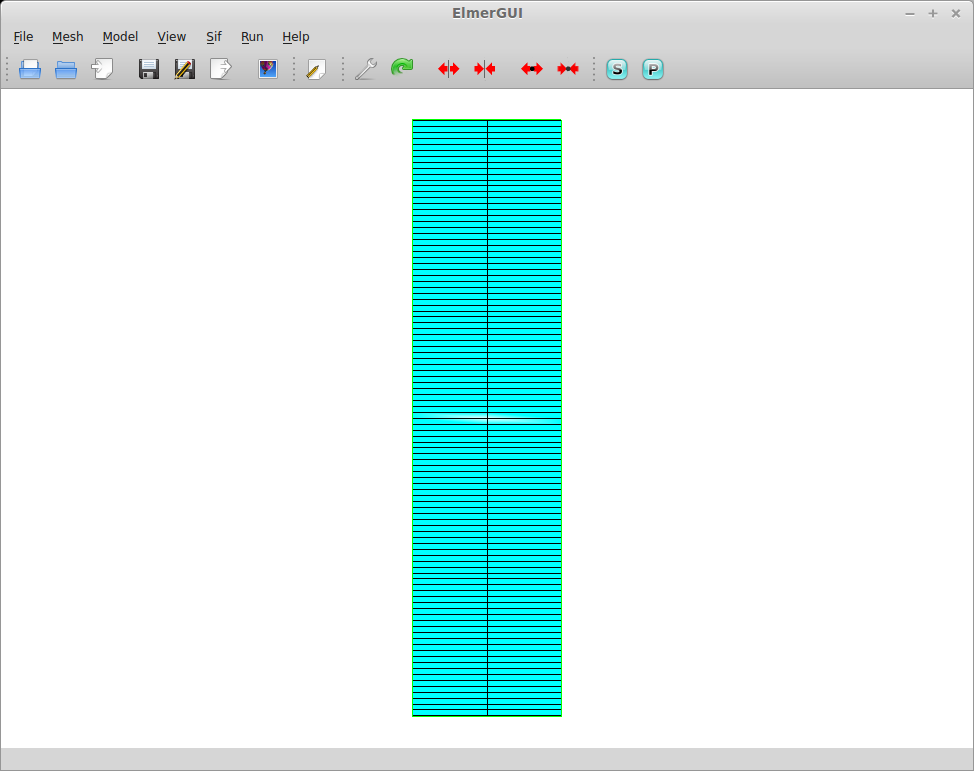
\includegraphics[width=100mm]{GeoSlabGeom}
\caption{The geometry of the mesh in ElmerGUI}\label{fg:geomesh}
\end{center}
\end{figure}

After we have the mesh we start to go through the Model menu from the top to bottom. 
In the \texttt{Setup} we choose things related to the whole simulation such as file names, 
time stepping, constants etc.
The simulation is carried out in 2-dimensional cartesian
coordinates and in transient. 
We will use 1000 timesteps each of size 10 years. 
For time-stepping we will use 2nd order scheme. 
\ttbegin
Model
  Setup 
    Simulation Type = Steady transient
    Timestepping Method = BDF
    Timestepping Order = 2 
    Timestep Intervals = 10000
    Timestep Sizes = $10*365*24*3600
    Output Intervals = 2
\ttend
Choose \texttt{Accept} to close the window.

In the equation section we choose the relevant equations and parameters related to their solution. 
In this case we'll have one set only one equation -- the heat equation.


When defining Equations and Materials it is possible to assign the to bodies immediately, or to use mouse
selection to assign them later. In this case we have just one body and one boundary and therefore its easier to assign 
the Equation and Material to it directly.

For the linear system solvers we are happy to use the defaults. One may however, try out different
preconditioners (ILU1,\ldots) or direct Umfpack solver, for example.
\ttbegin
Model
  Equation
    Add 
      Name = Heat Equation
      Apply to bodies = 1
      Heat Equation
        Active = on
  Apply   
  OK
\ttend        

The Material section includes all the material parameters.
They are divided to generic parameters which are direct properties of the material
without making any assumptions on the physical model, such as the mass. Other properties assume
a physical law, such heat conductivity.
\ttbegin
Model
  Material
    Add 
      Name = Granite
      Apply to bodies = 1 
      General    
        Density = 2700.0
        Heat Capacity = 1250.0
      Heat Equation
        Heat Conductivity = 2.5
    Apply
    OK
\ttend

We will need an initial condition for the case. 
\ttbegin
Model
  Initial Condition
    Add 
      Name = InitialState
      Heat Equation
        Temperature -> press enter and write the expression
      Apply to bodies = 1
    Apply
    OK
\ttend    
Now the expression to be written uses an internal linear interpolation feature of Elmer. 
\begin{verbatim}
Variable coordinate 2
  Real
    -8000 320.0
    -6500 260.0
    -6499 500.0
    -5501 500.0
    -5500 220.0
    -4000 160.0
  End
\end{verbatim}

In this case we only need boundary conditions for the upper and lower boundary.
First we create the boundary conditions
\ttbegin
Model
  BoundaryCondition
    Add 
      Heat Equation
        Temperature = 320.0
      Name = Down
      OK
    Add 
      Heat Equation
        Temperature = 160.0
      Name = Up
      OK
\ttend   
Then we set the boundary properties 
\ttbegin
Model 
  Set boundary properties  
\ttend
Choose the defined group of three boundaries by clicking with the mouse
and apply the condition for the lower boundary.
\ttbegin
Boundary condition
  Down
\ttend
and similarly for the upper boundary. 


For the execution 
ElmerSolver needs the mesh files and the command file. We have know basically defined
all the information for ElmerGUI to write the command file. After writing it we may also visually 
inspect the command file.
\ttbegin
Sif
  Generate
  Edit... -> look how your command file came out  
\ttend

Before we can execute the solver we should save the files in a directory. In saving the project all the
necessary files for restarting the case will be saved to the 
destination directory.
\ttbegin
File 
  Save Project
\ttend

After we have successfully saved the files we may start the solver
\ttbegin
Run
  Start solver
\ttend
A convergence view automatically pops up showing relative changes of each iteration.
As the case is linear only one iteration was required for the solution and the second one
just is needed to check the convergence. 
The resulting output log is shown in figure~\ref{fg:GeoSlabConv}.

\begin{figure}
\begin{center}
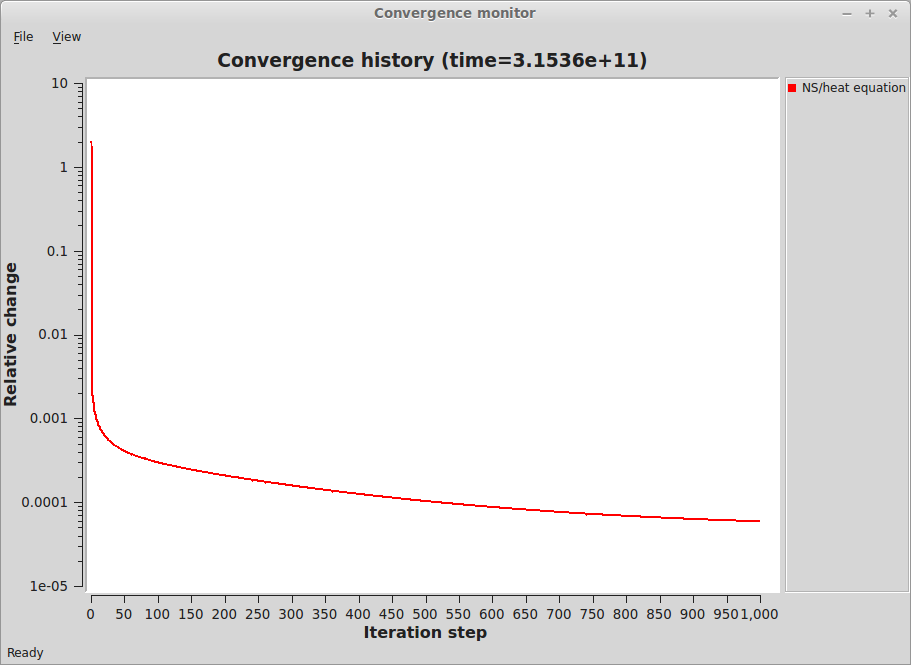
\includegraphics[width=100mm]{GeoSlabConvergence}
\caption{The output log of ElmerSolver when used under ElmerGUI}\label{fg:GeoSlabConv}
\end{center}
\end{figure}

Note: if you face problems in the solution phase and need to edit the setting, always remember to save
the project before execution.

To view the results we use Paraview.
\ttbegin
Run
  Start ParaView
\ttend
If your configuration is ok a Paraview window should pop up.
Choose temperature for the surface to be plotted. 
As we have a timeseries we may run the sequence by pressing the play icon. 

You may also choose the \texttt{Plot Over Line} filter to see the data plotted 
over a line for better numerical inspection. 

\begin{figure}
\begin{center}
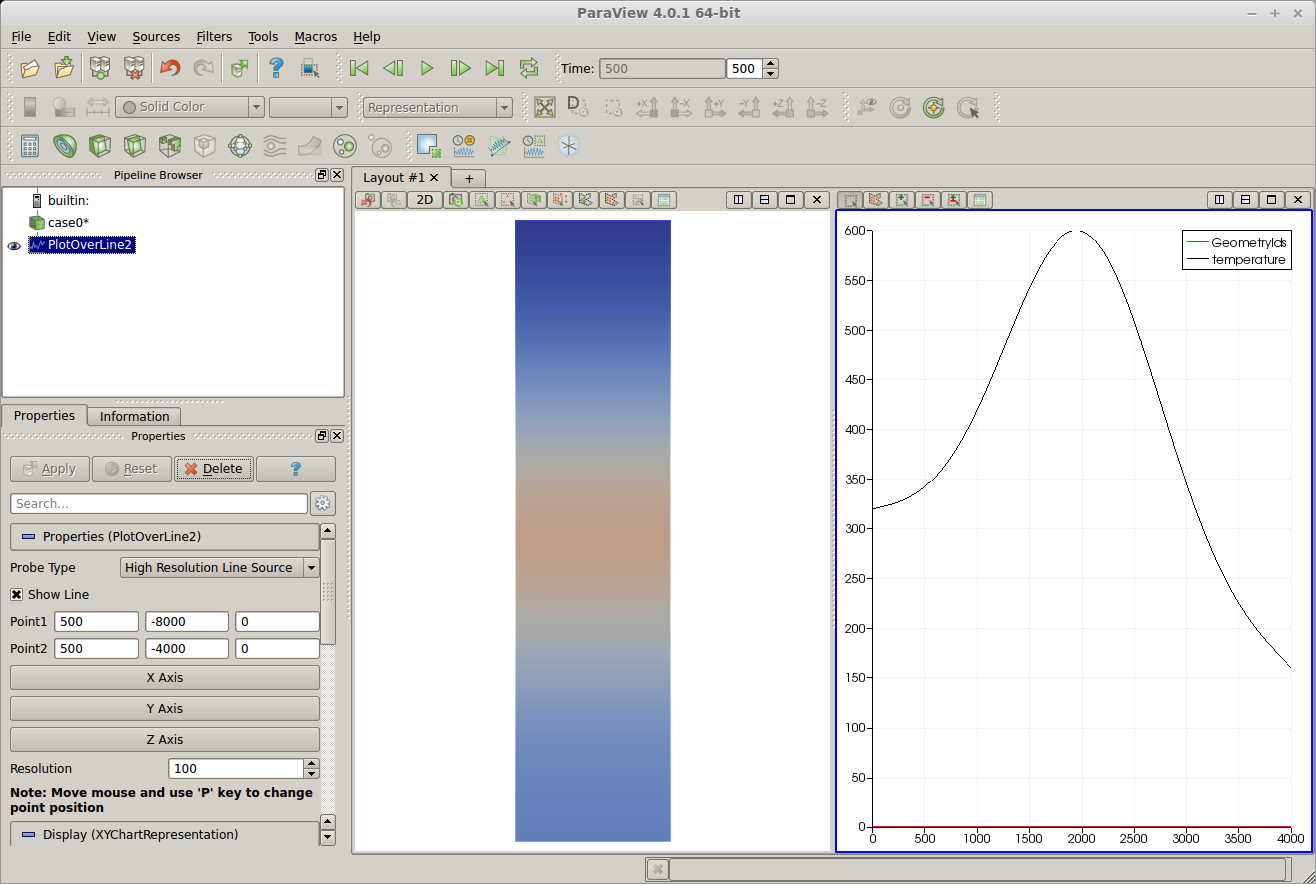
\includegraphics[width=140mm]{GeoSlabParaview}
\caption{The data visualized in Paraview as a surface and lineplot}
\label{fg:GeoSlabParaview}
\end{center}
\end{figure}

The final maximum temperature of the analysis is around 600~C. Whether this is close to correct could
be studied by increasing further the time and space resolution. 


\subsection{Variation accounting for latent heat release}

For intrusion processes the latent heat often plays on important role. 
For that the internal phase change model can be used. It requires that 
all the internal energy is expressed using specific enthalphy rather than
heat capacity and latent heat. 

We now eliminate the heat capacity of the original case (1250~J/kgK) and
create a specific enthalpy that includes heat capacity of 1000~J/kgJ 
and latent heat release of 200~kJ/kg release between interval 700--800 C.

The expression for \texttt{Specific Enthalpy} accounting for these two now yields
\begin{verbatim}
Variable Temperature
  Real
    0.0  0.0
    700  7.0e5
    800  9.0e5
    900  10.0e5
 End 
\end{verbatim}
For the phase change model we select 
\ttbegin
Model
  Equation
    Heat Equation
      Phase Change Model = spatial 2
  Update
  OK
\ttend        
With these changes the maximum temperature at the end of simulation cycle 
becomes around 624~C.  


\hfill
\mbox{}






